\task{Катим круг}
\begin{itemize}
\itA «Расправим» большую окружность — заметим, что дуга, составляющая её половину, равна по длине окружности круга, который мы катим. Это значит, что, проехав эту дугу, круг снова коснётся её отмеченной точкой.

\begin{center}
	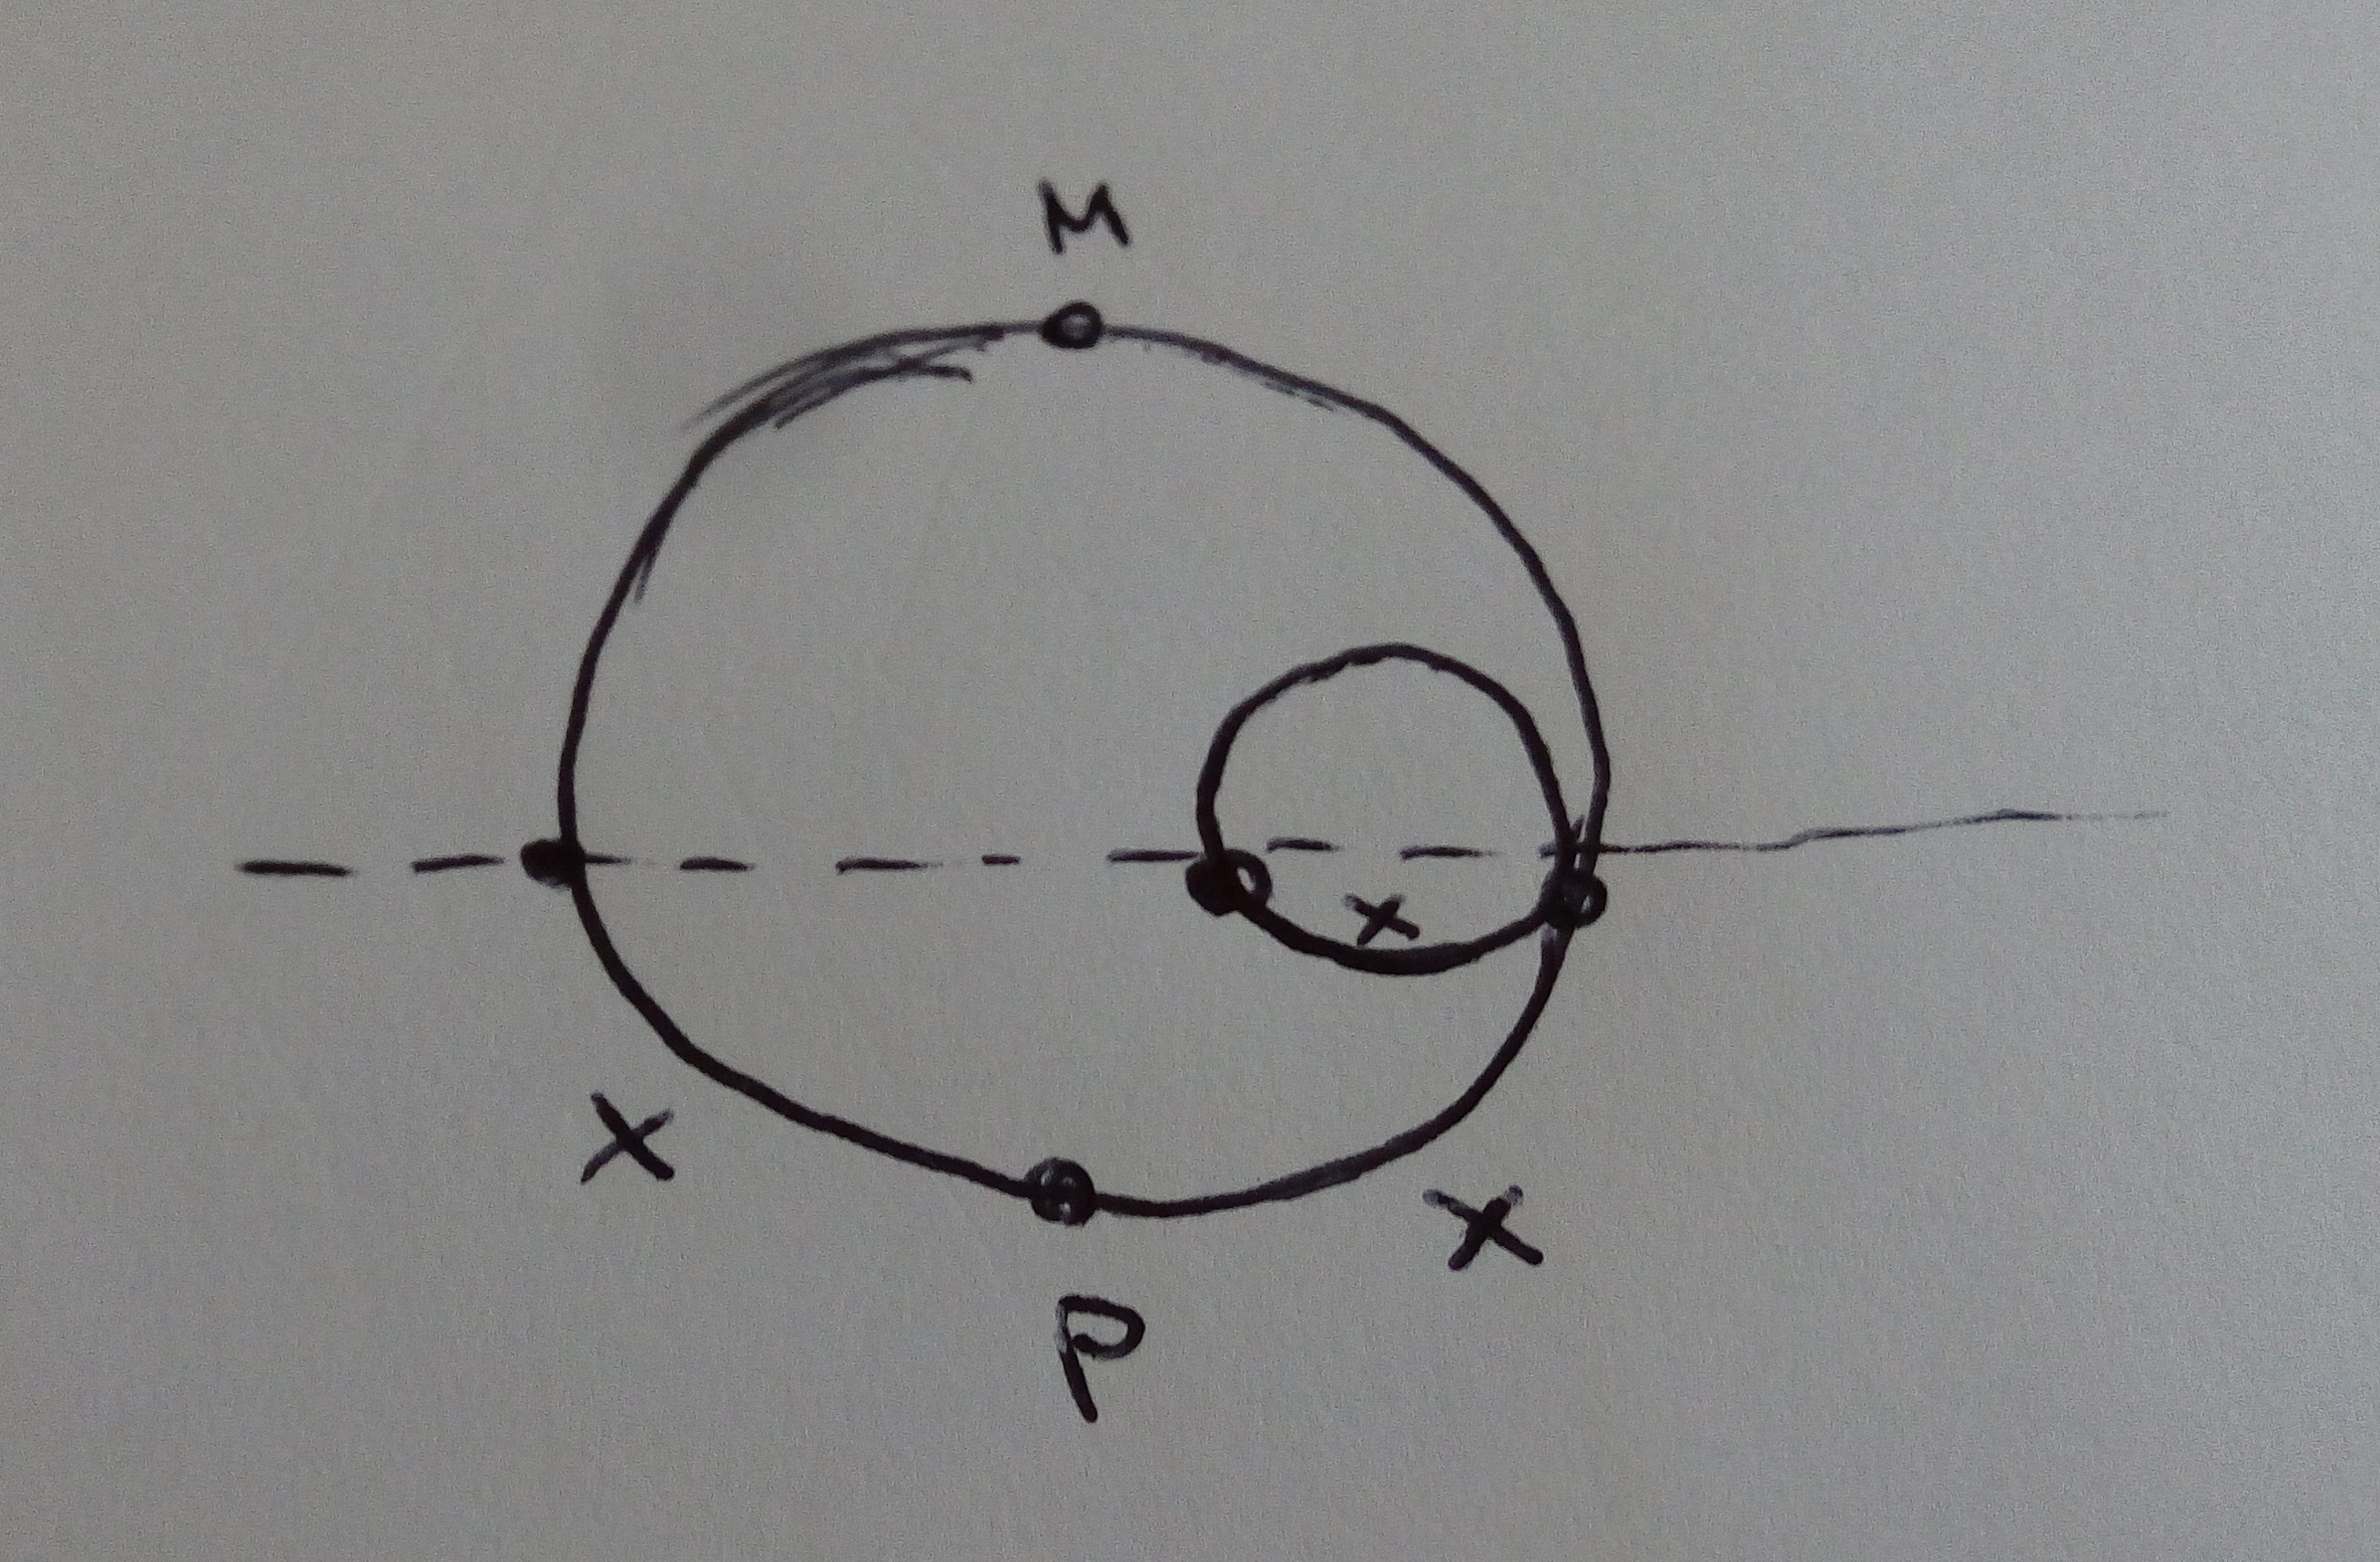
\includegraphics[natwidth=2614,natheight=1716,width=6cm]{figures/2018-circle-move}
\end{center}

\itB Длина дуги круга между точкой его касания с окружностью и отмеченной точкой равна длине дуги окружности между точкой её касания с кругом и точкой $P$. Обозначим эту длину через $x$. Отложим дугу длиной $x$ налево от точки $P$ (смотреть рисунок). Отрезок, соединяющий точку касания круга с окружностью и конец новой дуги, будет горизонтальным.

При этом дуга длины $x$ на круге получается из дуги длины $x$ на окружности гомотетией с коэффициентом $\tfrac{1}{2}$ и центром в точке касания круга с окружностью: эти дуги отложены из одной точки на окружностях, радиусы которых отличаются в два раза.

Горизонтальный отрезок переходит при гомотетии в горизонтальный отрезок — поэтому концы дуги на квадрате также лежат на одной горизонтальной прямой.

\itC В силу того же факта, что дуга на квадрате получается из дуги на окружности гомотетией с коэффициентом $\tfrac{1}{2}$, её конец будет находится ровно посередине между концами большой дуги — то есть, ровно над точкой $P$, потому как большая дуга изначально строилась симметричной.
\end{itemize}